\chapter{Uncertainties and Validation}
\label{chap:bbbb-uncert}

A variety of uncertainties are assigned to account for known biases in the
underlying methods, calibrations, and objects used for this analysis. The
largest such uncertainty is associated with the kinematic bias inherent in
deriving the background estimate outside of the signal region. However, a
statistical biasing of this same estimate also has a significant impact.
Additionally, due to the use of Monte Carlo for signal modelling and \btag
calibration, uncertainties related to mis-modelings in simulation must also be
accounted for. Note that the results for the non-resonant analysis presented here are 
preliminary and only include background systematic, such that the discussion of the 
signal systematics \emph{only} applies for the resonant search. However, these background 
systematics are expected to be by far the dominant uncertainties.

\section{Statistical Uncertainties and Bootstrapping}
There are two components to the statistical error for the neural network
background estimate. The first is standard Poisson error, i.e., a given bin,
$i$, in the background histogram has value $n_i = \sum\limits_{j\in i} w_j$,
where $w_j$ is the weight for an event $j$ which falls in bin $i$. Standard
techniques then result in statistical error $\delta n_i =
	\sqrt{\sum\limits_{j\in i} w_j^2}$, which reduces to the familiar $\sqrt{N}$
Poisson error when all $w_j$ are equal to 1.

However, this procedure does not take into account the statistical uncertainty
on the $w_j$ due to the finite training dataset. Due to the large size
difference between the two tag and four tag datasets, it is the statistical
uncertainty due to the four tag training data that dominates that on the
background. A standard method for estimating this uncertainty is the bootstrap
resampling technique~\cite{Bootstrap}. Conceptually, a set of statistically
equivalent sets is constructed by sampling with replacement from the original
training set. The reweighting network is then trained on each of these
separately, resulting in a set of statistically equivalent background estimates.
Each of these sets is below referred to as a replica.

In practice, as the original training set is large, the resampling procedure is
able to be simplified through the relation $\lim\limits_{n\rightarrow \infty}
	\operatorname{Binomial}(n, 1/n) = \operatorname{Poisson}(1)$, which dictates that sampling
with replacement is approximately equivalent to applying a randomly distributed
integer weight to each event, drawn from a Poisson distribution with a mean of
1.

Though the network configuration itself is the same for each bootstrap training, the
network initialization is allowed to vary. It should therefore be noted that the bootstrap
uncertainties implicitly capture the uncertainty due to this variation in addition to
the previously mentioned training set variation.

The variation from this bootstrapping procedure is used to assign a bin-by-bin uncertainty
which is treated as a statistical uncertainty in the fit. Due to practical constraints,
a procedure for approximating the full bootstrap error band is developed which demonstrates
good agreement with the full bootstrap uncertainty. This procedure is described below.

\subsection{Calculating the Bootstrap Error Band}
The standard procedure to calculate the bootstrap uncertainty would proceed as 
follows: first, each network trained on each bootstrap replica dataset would be used
to produce a histogram in the variable of interest. This would result in a set of 
replica histograms (e.g. for 100 bootstrap replicas, 100 histograms would be created). 
The nominal estimate would then be the mean of bin values across these replica histograms, 
with errors set by the corresponding standard deviation.

In practice, such an approach is inflexible and demanding both in computation and 
in storage, in so far as we would like to produce histograms in many variables, with a 
variety of different cuts and binnings. This motivates a derivation based on event-level 
quantities. However, due to non-trivial correlations between replica weights, simple linear 
propagation of event weight variation is not correct.

We therefore adopt an approach which has been empirically found to produce results (for this
analysis) in line with those produced by generating all of the histograms, as in the standard 
procedure. This approach is described below. Note that, for robustness to outliers and weight distribution 
asymmetry, the median and interquartile range (IQR) are used for the central value and width 
respectively (as opposed to the mean and standard deviation).

The components involved in the calculation have been mentioned in Chapter \ref{chap:bbbb-background} and 
are as follows:
\begin{enumerate}
\item Replica weight ($w_{i}$): weight predicted for a given event by a network trained on replica 
dataset $i$.
\item Replica norm ($\alpha_{i}$): normalization factor for replica $i$. This normalizes the reweighting 
prediction of the network trained on replica dataset $i$ to match the corresponding target yield.
\item Median weight ($w_{med}$): median weight for a given event across replica datasets, used for the nominal estimate. Defined (for 100 bootstrap replicas) as
\begin{equation}
w_{med} \equiv \operatorname{median}(\alpha_{1}w_{1}, \ldots \alpha_{100}w_{100})
\end{equation}
\item Normalization correction ($\alpha_{med}$): normalization factor to match the predicted yield of the median weights
($w_{med}$) to the target yield in the training region.
\end{enumerate}

As mentioned in Chapter \ref{chap:bbbb-background}, the \emph{nominal estimate} is constructed from the set of
median weights and the normalization correction, i.e. $\alpha_{med}\cdot w_{med}$.

For the bootstrap error band, a ``varied'' histogram is then generated by applying, for each event, a weight
equal to the median weight (with no normalization correction) plus half the interquartile range of 
the replica weights: $w_{varied} = w_{med} + \frac{1}{2}\operatorname{IQR}(w_{1},\ldots, w_{100})$.

This varied histogram is scaled to match the yield of the nominal estimate. To account for variation of the 
nominal estimate yield, a normalization variation is calculated from the interquartile range of the replica norms:
$\frac{1}{2}\operatorname{IQR}(\alpha_{1}, \ldots, \alpha_{100})$. This variation, multiplied into the nominal
estimate, is used to set a baseline for the varied histogram described above.

Denoting $H$(weights) as a histogram constructed from a given set of weights, $Y$(weights) as the predicted yield
for a given set of weights, the final varied histogram is thus:
\begin{equation}
H(w_{med} +\frac{1}{2}\operatorname{IQR}(w_{1},\ldots, w_{100}))\cdot \frac{Y(\alpha_{med}w_{med})}{Y(w_{med} +\frac{1}{2}\operatorname{IQR}(w_{1},\ldots, w_{100}))} + \frac{1}{2}\operatorname{IQR}(\alpha_{1}, \ldots, \alpha_{100})\cdot H(\alpha_{med}w_{med})
\end{equation}

where the first term roughly describes the behavior of the bootstrap variation across the distribution of 
the variable of interest while the second term describes the normalization variation of the bootstrap replicas.

The difference between the varied histogram and the nominal histogram is then
taken to be the bootstrap statistical uncertainty on the nominal histogram.

Figure \ref{fig:bootstrap-breakdown} demonstrates how each of the components described above
contribute to the uncertainty envelope for the non-resonant 2017 Control Region 
and compares this approximate band to the variation of histograms from individual bootstrap 
estimates. The error band constructed from the above procedure is seen to provide a good 
description of the bootstrap variation.

\begin{figure}[ht]
	\centering
	\subfloat[IQR varied histogram (before normalizing)]{\label{fig:bstrap-IQR-hist}%
		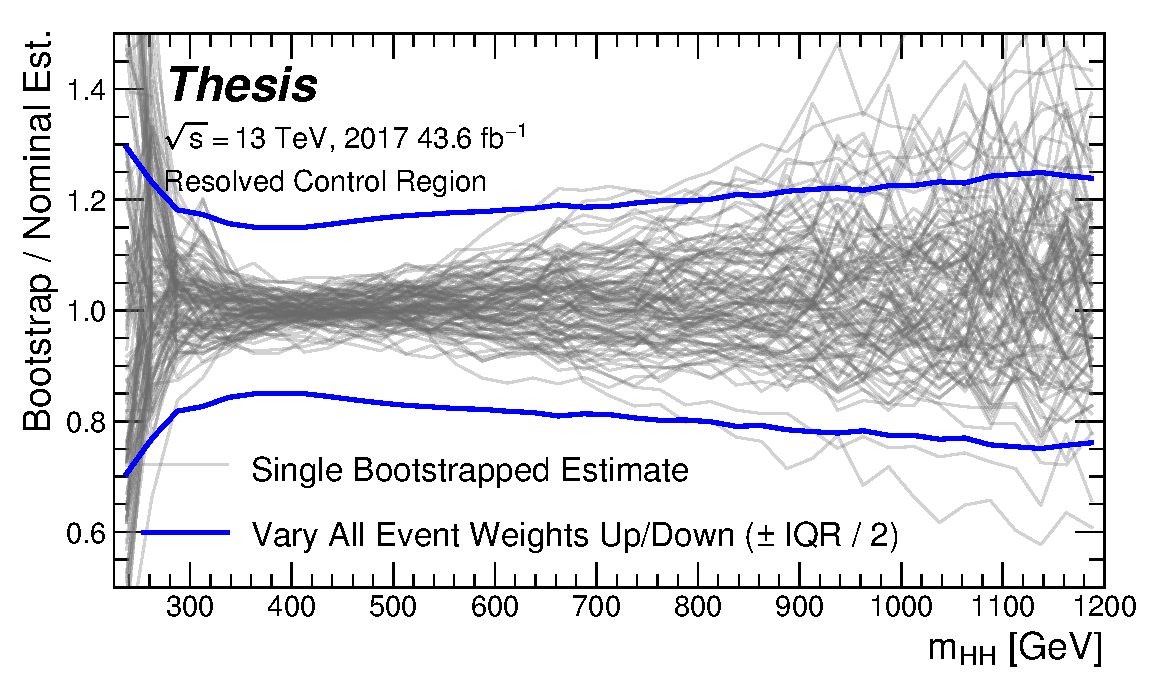
\includegraphics[width=0.48\textwidth]{figures/thesis-Xhh-45-bootstrap-exp-plots-weightIQR-up-down-2017-CR.pdf}
	}
	\subfloat[Normalization correction]{\label{fig:bstrap-norm}%
		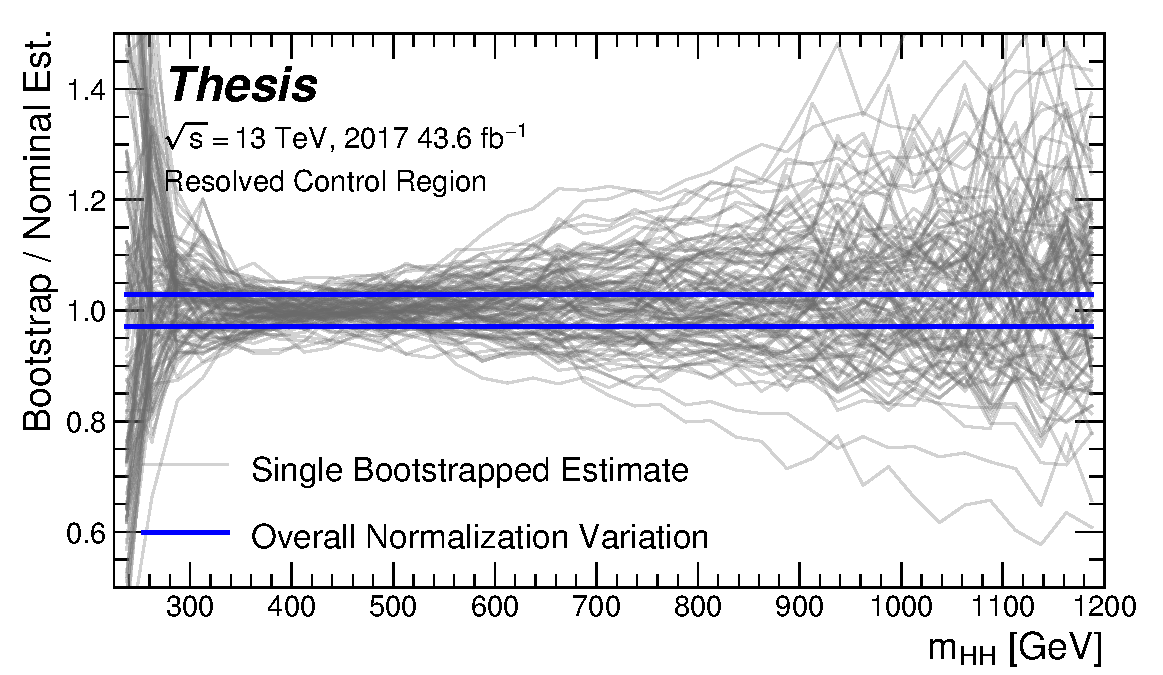
\includegraphics[width=0.48\textwidth]{figures/thesis-Xhh-45-bootstrap-exp-plots-norm-up-down-2017-CR.pdf}
	}

	\subfloat[Final bootstrap error band]{\label{fig:bstrap-band}%
		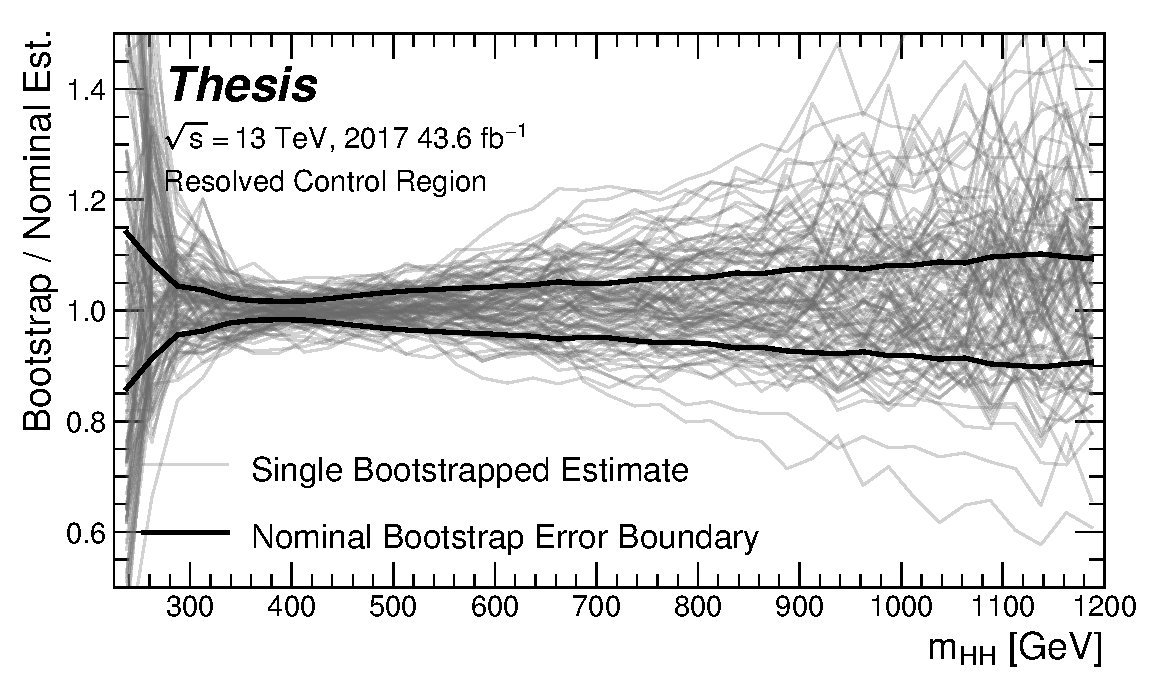
\includegraphics[width=0.48\textwidth]{figures/thesis-Xhh-45-bootstrap-exp-plots-nominal-band-2017-CR.pdf}
	}
	\subfloat[Comparison with histogram bin IQR]{\label{fig:bstrap-band-vs-hist-iqr}%
		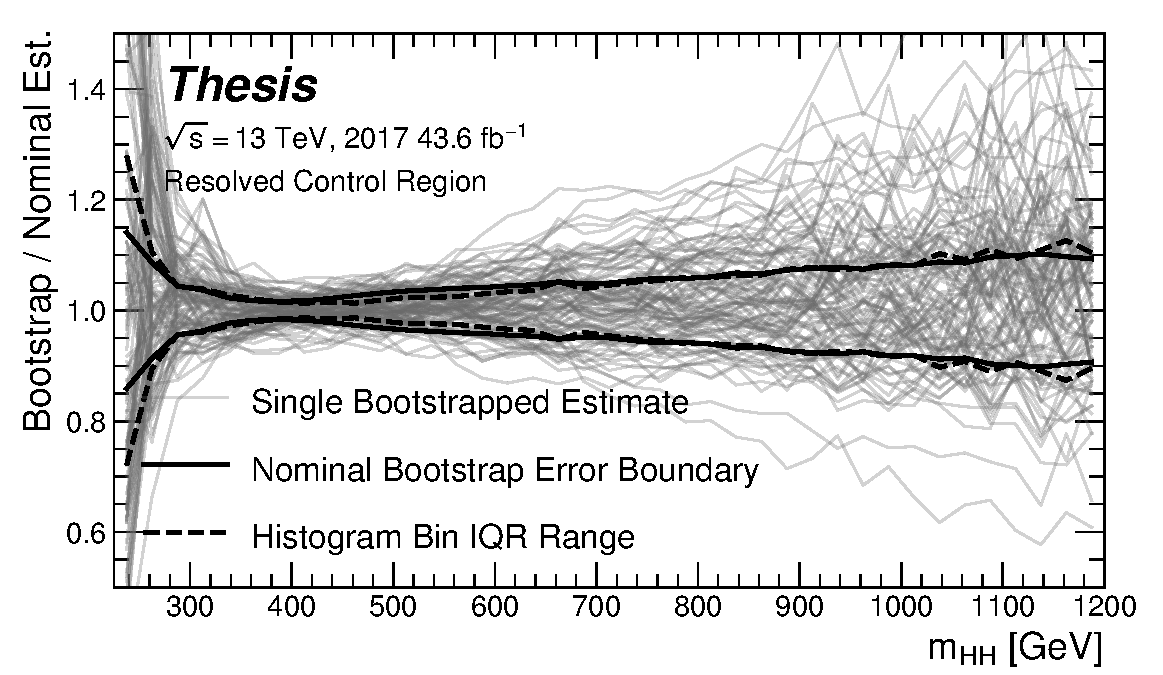
\includegraphics[width=0.48\textwidth]{figures/thesis-Xhh-45-bootstrap-exp-plots-nominal-band-compare-with-hist-IQR-2017-CR.pdf}
	}

	\caption{Illustration of the approximate bootstrap band procedure, shown as a ratio to the nominal estimate 
	for the 2017 non-resonant background estimate. Each grey line is from the \mhh prediction for a 
	single bootstrap training. Figure \ref{fig:bstrap-IQR-hist} shows 
	the variation histograms constructed from median weight $\pm$ the IQR of the replica weights. It can be seen 
	that this captures the rough shape of the bootstrap envelope, but is not good estimate for the overall magnitude
	of the variation. Figure \ref{fig:bstrap-norm} demonstrates the applied normalization correction, and Figure 
	\ref{fig:bstrap-band} shows the final band (normalized Figure \ref{fig:bstrap-IQR-hist} + 
	Figure \ref{fig:bstrap-norm}). Comparing this with the IQR variation for the prediction from each bootstrap 
	in each bin in Figure \ref{fig:bstrap-band-vs-hist-iqr}, the approximate envelope describes a very similar variation.}
	\label{fig:bootstrap-breakdown}
\end{figure}

\FloatBarrier
\section{Background Shape Uncertainties}
To account for the systematic bias associated with deriving the reweighting function
in the control region and extrapolating to the signal region, an alternative background
model is derived in the validation region. Because of the fully data-driven nature of the 
background model, this is an uncertainty assessed on the full background. The alternative model 
and the baseline are consistent with the observed data in their training regions, and 
differences between the alternative and baseline models are used to define a shape uncertainty on the \mhh
spectrum, with a two-sided uncertainty defined by symmetrizing the difference about
the baseline.

For the resonant analysis, this uncertainty is split into two components to allow for two 
independent variations of the \mhh spectrum: a low-$H_{T}$ and a high-$H_{T}$ component,
where $H_{T}$ is the scalar sum of the $p_{T}$ of the four jets constituting the
Higgs boson candidates, and serves as a proxy for \mhh, while avoiding
introducing a sharp discontinuity. The boundary value is \SI{300}{\GeV}. The
low-$H_{T}$ shape uncertainty primarily affects the \mhh spectrum below
\SI{400}{\GeV} (close to the kinematic threshold) by up to around 5\%, and the
high-$H_{T}$ uncertainty mainly \mhh above this by up to around 20\% relative to
nominal. These separate \mhh regimes are by design -- the $H_{T}$ split is 
introduced to prevent low mass bins from constraining the high mass uncertainty 
and vice-versa. 

This was the \emph{status quo} shape uncertainty decomposition from the
Early~Run~2 analysis. A decomposition in terms of orthogonal polynomials, which
would provide increased flexibility, was also evaluated. This study revealed
that both decompositions are able to account for the systematic deviations
between four tag data and the background estimate (evaluated in the kinematic
validation region), and produce almost identical limits. The simpler \emph{status quo} decomposition 
is therefore kept.

For the non-resonant analysis, the quadrant nature of the background estimation
leads to a natural breakdown of the nuisance parameters: quadrants are defined 
in the signal region along the same axes as those used for the control and validation 
region definitions. Variations are then assessed in each of these signal region quadrants,
corresponding to regions that are ``closer to'' and ``further away from'' the 
nominal and alternate estimate regions, fully leveraging the power of the two
equivalent but systematically different estimates.

Figure \ref{fig:res-shapesyst-var-18} shows an example of the variation in each 
$H_{T}$ region for the 2018 resonant analysis. Figure \ref{fig:nonres-shapesyst-var-18}
shows the example quadrant variation for the 2018 $4b$ non-resonant analysis.
\begin{figure}[ht]
	\centering
	\subfloat[Low $H_{T}$]{\label{fig:lowHT-shapesyst-18}%
		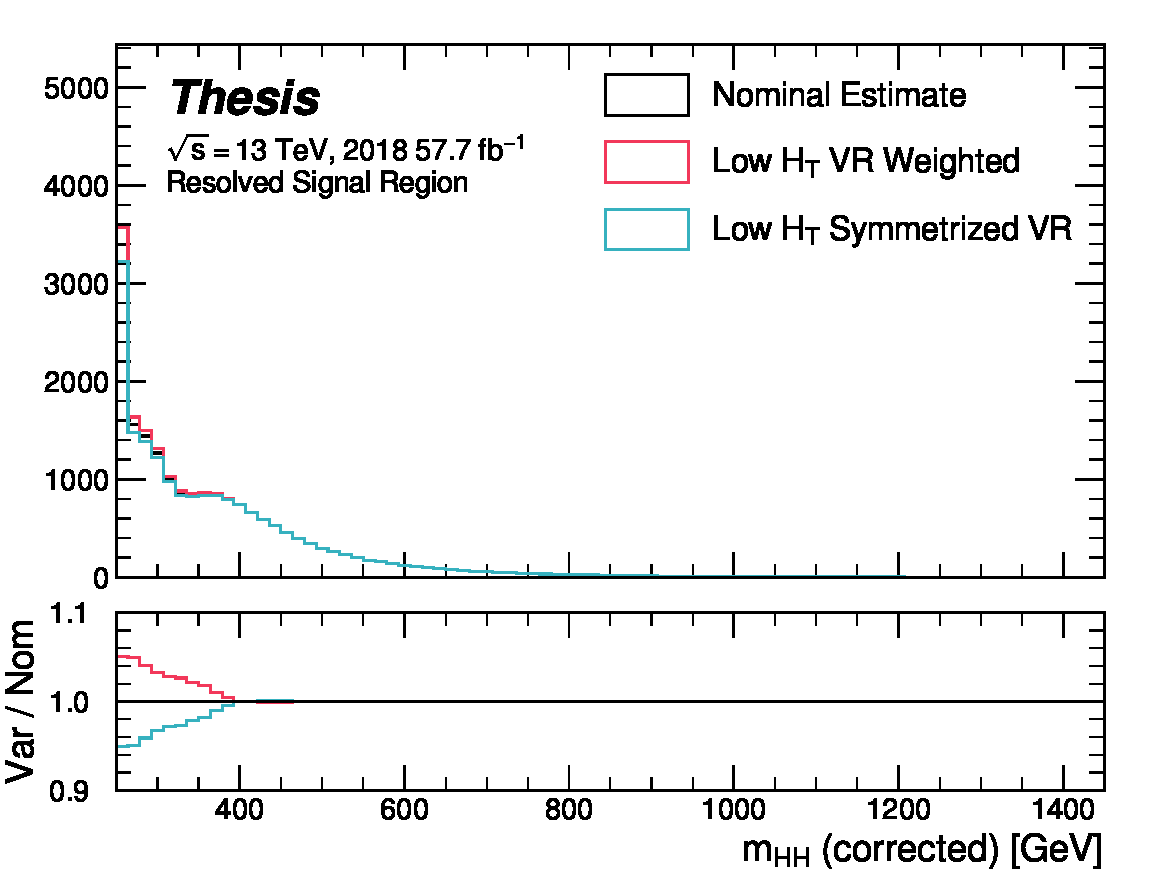
\includegraphics[width=0.48\textwidth]{figures/thesis-res-lowHT-HTsplit-syst-m-hh-cor-Signal-NN-18-4b.pdf}
	}
	\subfloat[High $H_{T}$]{\label{fig:highHT-shapesyst-18}%
		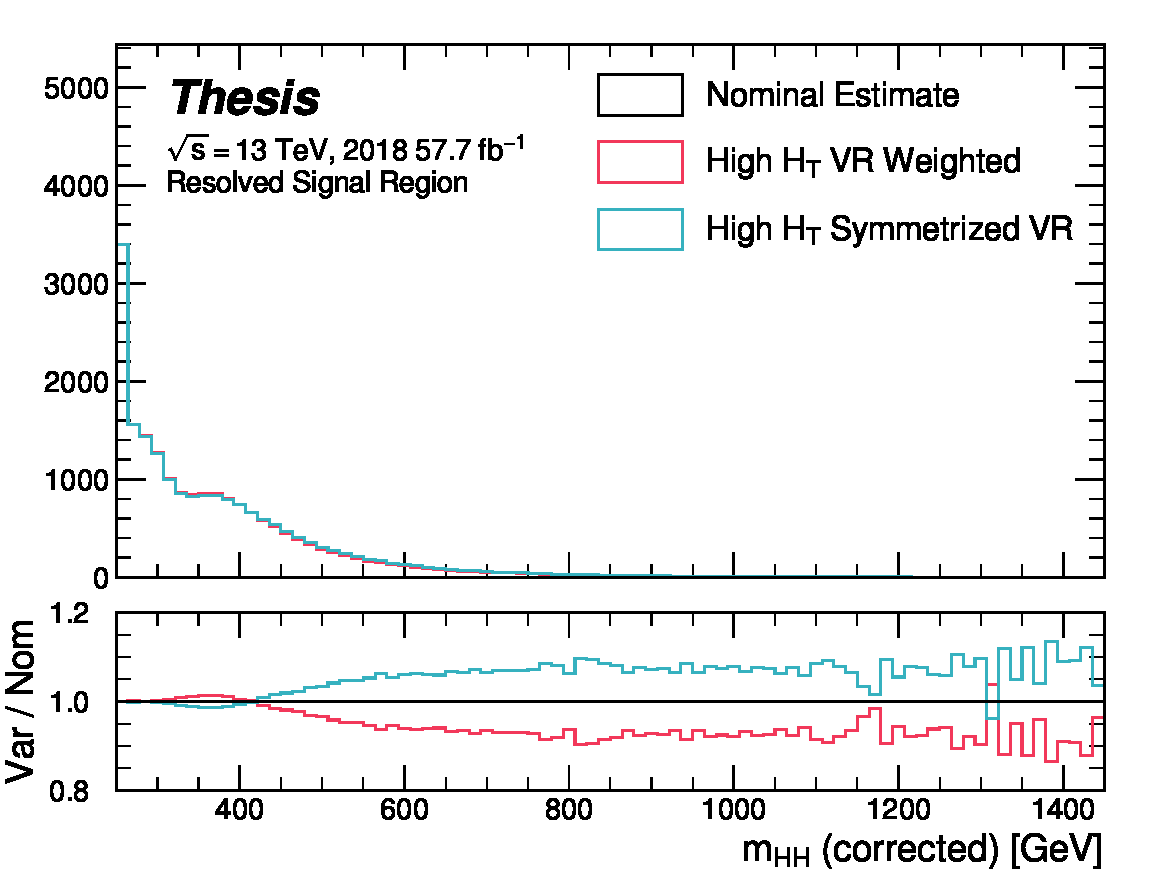
\includegraphics[width=0.48\textwidth]{figures/thesis-res-highHT-HTsplit-syst-m-hh-cor-Signal-NN-18-4b.pdf}
	}
	\caption{\textbf{Resonant Search}: Example of CR vs VR variation in each $H_{T}$ region 
	for 2018. The variation nicely factorizes into low and high mass components.}
	\label{fig:res-shapesyst-var-18}
\end{figure}
\begin{figure}[ht]
	\centering
	\vspace*{-3cm}
	\subfloat[Q1 (top)]{\label{fig:Q1-shapesyst-18}%
		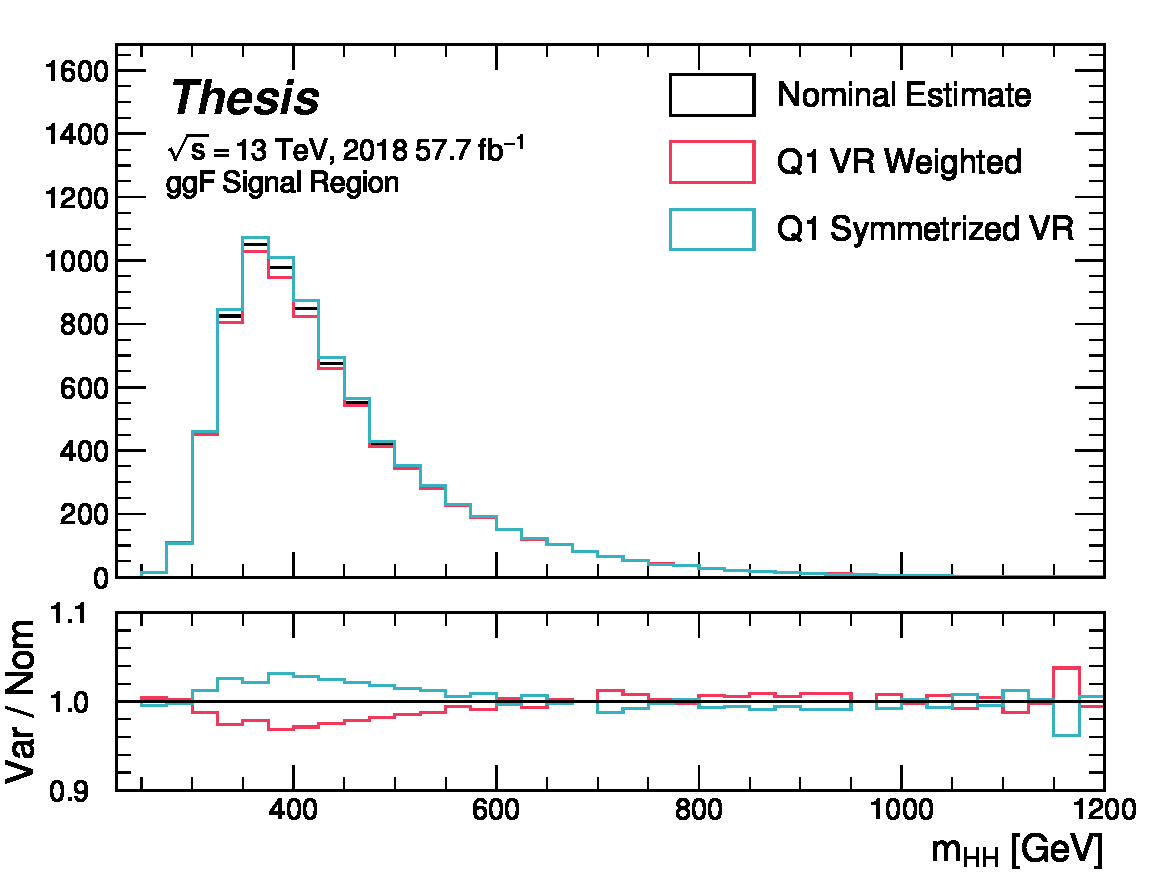
\includegraphics[width=0.48\textwidth]{figures/thesis-SR-Q1-SR-quads-rot-Xhh-syst-m-hh-Signal-NN-18-4b.pdf}
	}

	\subfloat[Q2 (left)]{\label{fig:Q2-shapesyst-18}%
		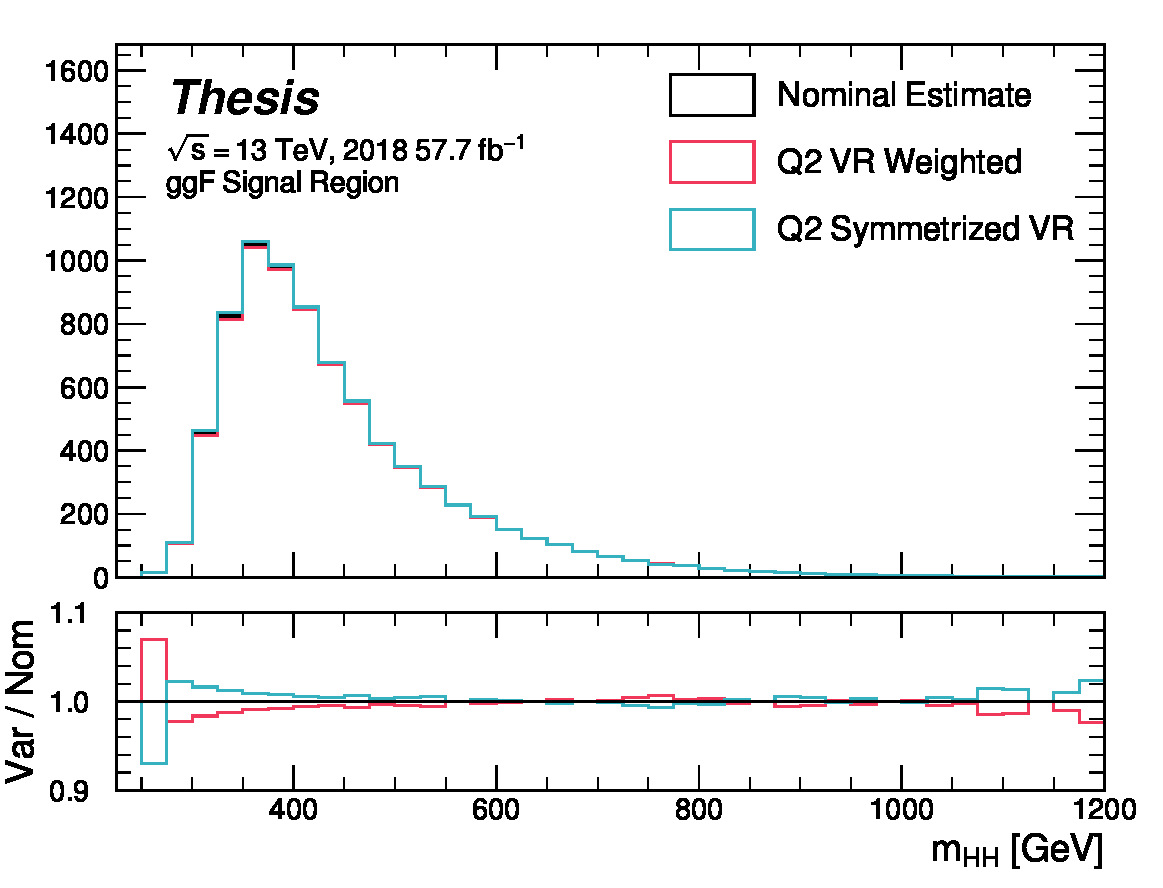
\includegraphics[width=0.48\textwidth]{figures/thesis-SR-Q2-SR-quads-rot-Xhh-syst-m-hh-Signal-NN-18-4b.pdf}
	}
	\subfloat[Q4 (right)]{\label{fig:Q4-shapesyst-18}%
		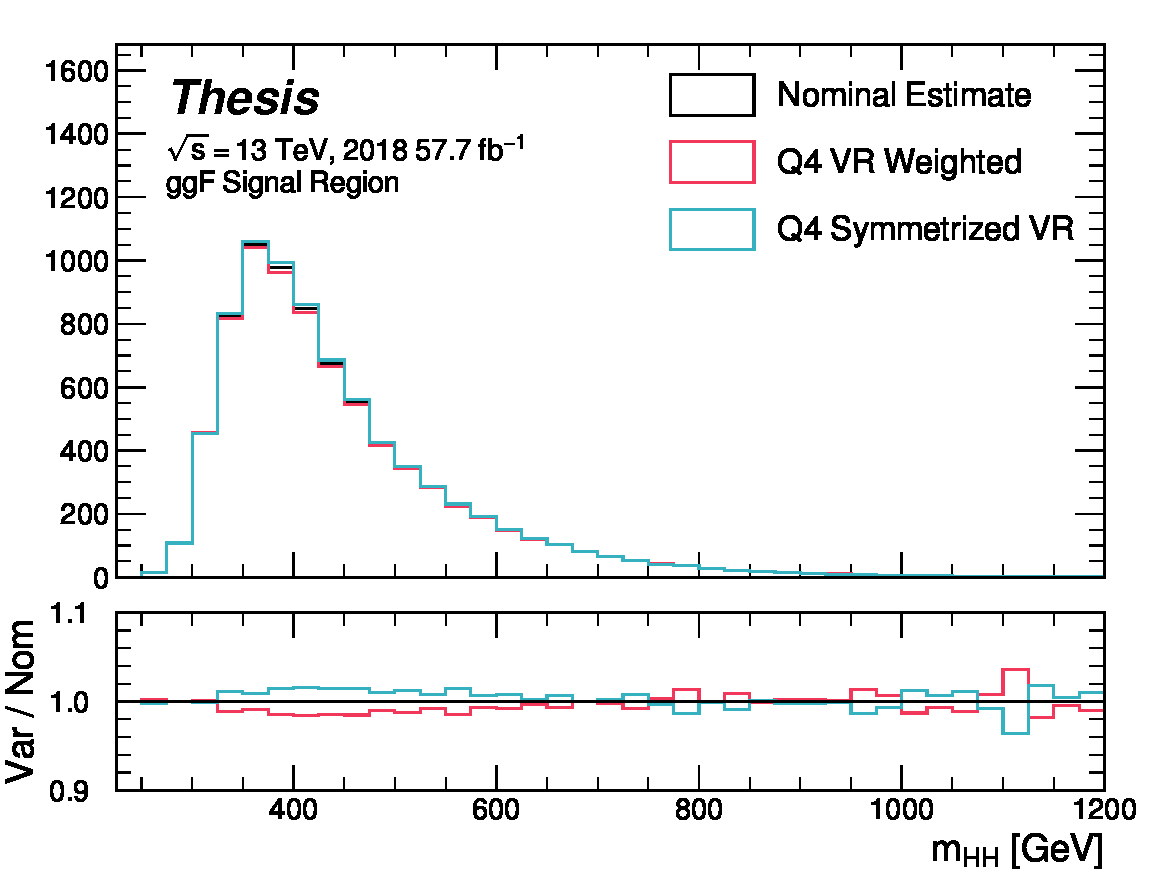
\includegraphics[width=0.48\textwidth]{figures/thesis-SR-Q4-SR-quads-rot-Xhh-syst-m-hh-Signal-NN-18-4b.pdf}
	}

	\subfloat[Q3 (bottom)]{\label{fig:Q3-shapesyst-18}%
		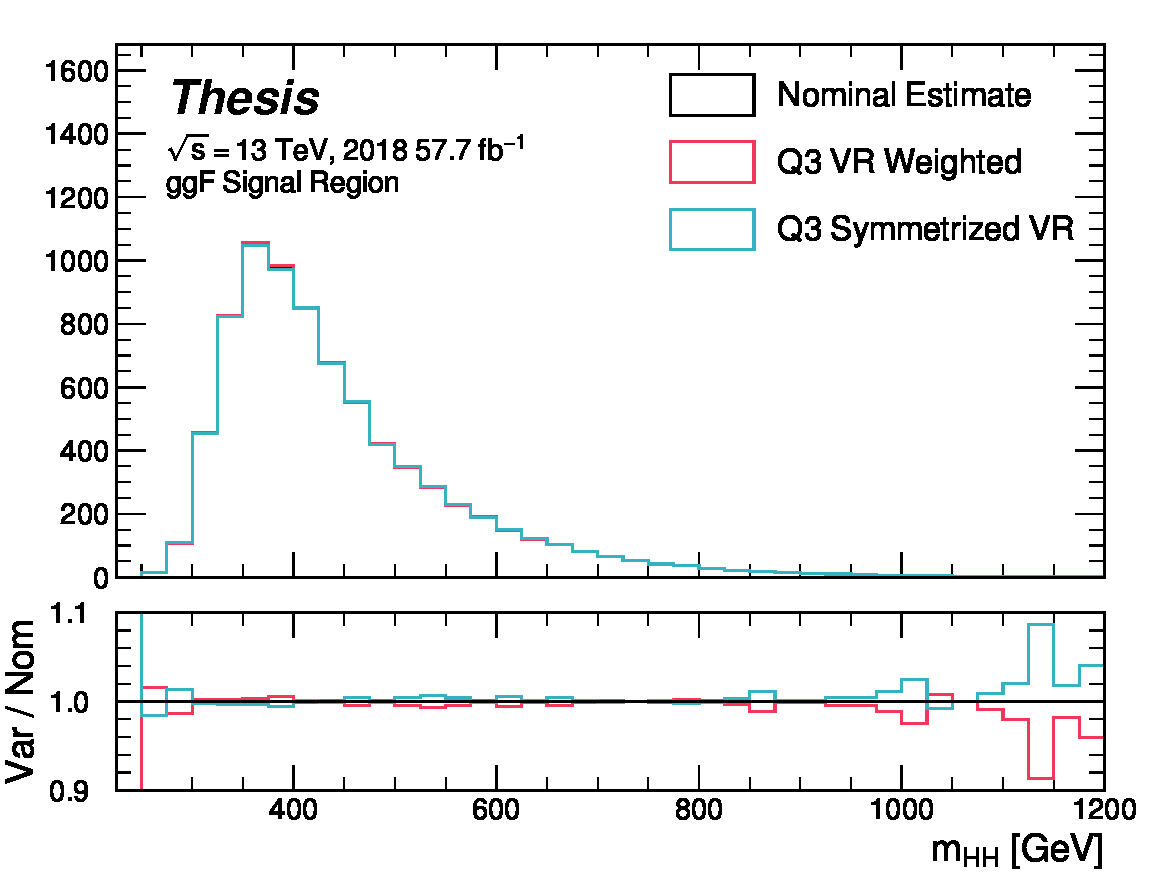
\includegraphics[width=0.48\textwidth]{figures/thesis-SR-Q3-SR-quads-rot-Xhh-syst-m-hh-Signal-NN-18-4b.pdf}
	}
	\caption{\textbf{Non-resonant Search (4b)}: Example of CR vs VR variation in each signal region quadrant 
	for 2018. Significantly different behavior is seen between quadrants, with the largest variation in quadrant 
	1 and the smallest in quadrant 4. \label{fig:nonres-shapesyst-var-18}}
\end{figure}

\FloatBarrier
\section{Signal Uncertainties}%
\label{sec:modelling-uncerts}
A variety of uncertainties are assessed on the the signal Monte Carlo simulation.  
As the background estimate is fully data driven, such uncertainties are not needed for 
the background estimate. Note again that the results presented for the non-resonant search only 
include the background systematics described above.

Detector modeling and reconstruction uncertainties account for differences 
between Monte Carlo simulation and real data due to mis-modeling of the detector
as well as due to the different performance of algorithms on simulation compared to data. 
In this analysis they consist of uncertainties related to jet properties and uncertainties stemming 
from the flavor tagging procedure. The jet uncertainties are treated according to the prescription in 
~\cite{JETM-2018-05} and are implemented as variations of the jet properties. These cover 
uncertainty in jet energy scale and resolution. Uncertainties in $b$-tagging efficiency are 
treated according to the prescription in Ref.~\cite{FTAG-2018-01} and implemented 
as scale factors applied to the Monte Carlo event weights. A systematic related to the PtReco \bjet 
energy correction has been studied in the \HepProcess{\higgs\higgs \to \gamma\gamma\Pqb\Paqb} 
analysis~\cite{bbyyNote} and found to be negligible compared to the other jet uncertainties. Following this 
example, such a systematic is therefore neglected here.

Trigger uncertainties stem from imperfect knowledge of the ratio between the
efficiency of a given trigger in data to its efficiency in Monte Carlo
simulation. This ratio is applied as a scale factor to all simulated events, with the 
systematic variations produced by varying the scale factor up or down by one sigma.
Such variations are evaluated based on measurements of per-jet online efficiencies for both jet reconstruction 
and $b$-tagging, and these are used to compute event-level uncertainties.
These are then applied as overall weight variations on the simulated events.

An uncertainty on the total integrated luminosity used in this analysis is also applied, 
ans is measured to be 1.7\%~\cite{ATLAS-CONF-2019-021}, obtained using the LUCID-2 detector for 
the primary luminosity measurements~\cite{Avoni:2633501}.

A variety of theoretical uncertainties are also assessed on the signal. Such uncertainties 
are assessed by generating samples following the configuration of the baseline samples,
but with modifications to probe various aspects of the simulation. These include
uncertainties in the parton density functions (PDFs); uncertainties due to
missing higher order terms in the matrix elements; and uncertainties in the
modelling of the underlying event, which includes multi-parton interactions, of
hadronic showers and of initial and final state radiation. 

Uncertainties due to modelling of the parton shower and the underlying event are 
evaluated by comparing results from using two different generators, namely \HERWIG[7.1.3]
and \PYTHIA[8.235]. No significant dependence on the variable of interest, \mhh, is observed.
Therefore, a 5\% flat systematic uncertainty is assigned to all signal samples, extracted from 
the acceptance comparison for the full 4-tag selection.

Uncertainties in the matrix element calculation are evaluated by varying the factorization 
and renormalization scales used in the generator up and down by a factor of two, both independently and simultaneously.
This results in an effect smaller than 1\% for all variations and all masses; the impact of such uncertainties 
is therefore neglected.

PDF uncertainties are evaluated using the PDF4LHC\_NLO\_MC set~\cite{Butterworth:2015oua} by 
calculating the signal acceptance for each PDF replica and taking the standard deviation. 
In all cases, these uncertainties result in an effect smaller than 1\% on the signal acceptance; 
therefore these are also neglected.

Theoretical uncertainties on the $H \to b\bar{b}$ branching ratio~\cite{deFlorian:2227475} are also 
included.

\FloatBarrier
\clearpage
\section{Background Validation}
\label{sec:bkgd-validation}
In addition to checking the performance of the background estimate in the control and 
validation regions, a variety of alternative selections are defined to allow for a 
full ``dress rehearsal'' of the background estimation procedure. 

Both the resonant and non-resonant analyses make use of a \emph{reversed $\Delta \eta$}
region, in which the kinematic cut on $\Delta \eta_{HH}$ is reversed, so that events are
required to have $\Delta \eta_{HH} > 1.5$. This is orthogonal to the nominal signal 
region and has minimal sensitivity, allowing for the comparison of the background
estimate $4b$ data in the corresponding ``signal region''. For this validation, 
a new reweighting is trained following nominal procedures, but entirely in the 
$\Delta \eta_{HH} > 1.5$ region. An example of such a validation is shown for the 
resonant search in Figure \ref{fig:res-rev-deta}.

The non-resonant analysis additionally makes use of the $3b+1$ fail region mentioned 
above, which again is orthogonal to the nominal signal regions and has minimal sensitivity.
The reweighting in this case is between $2b$ and $3b+1$ fail events rather than between 
$2b$ and $3b+1$ loose or $2b$ and $4b$. However, the kinematic selections of signal 
region events are otherwise identical, allowing for a complementary test of the 
background estimate. This validation is shown in Figure \ref{fig:nonres-sr-mhh-3b1f}.

Additional validation regions are also being explored, including those based on shifting the 
position of the set of analysis regions in the Higgs candidate mass plane and rederiving 
the background estimate in these shifted regions. Though each of these validations is different 
in some way from the set of regions in which the analysis is performed, evaluation of the performance 
of the background estimate in these regions is useful for developing and gaining confidence in the 
background estimation method and the corresponding uncertainties. Non-closure of the method in such 
regions may additionally be used for assessing uncertainties, but this is not considered here.

\begin{figure}[ht]
	\centering
	\subfloat{
		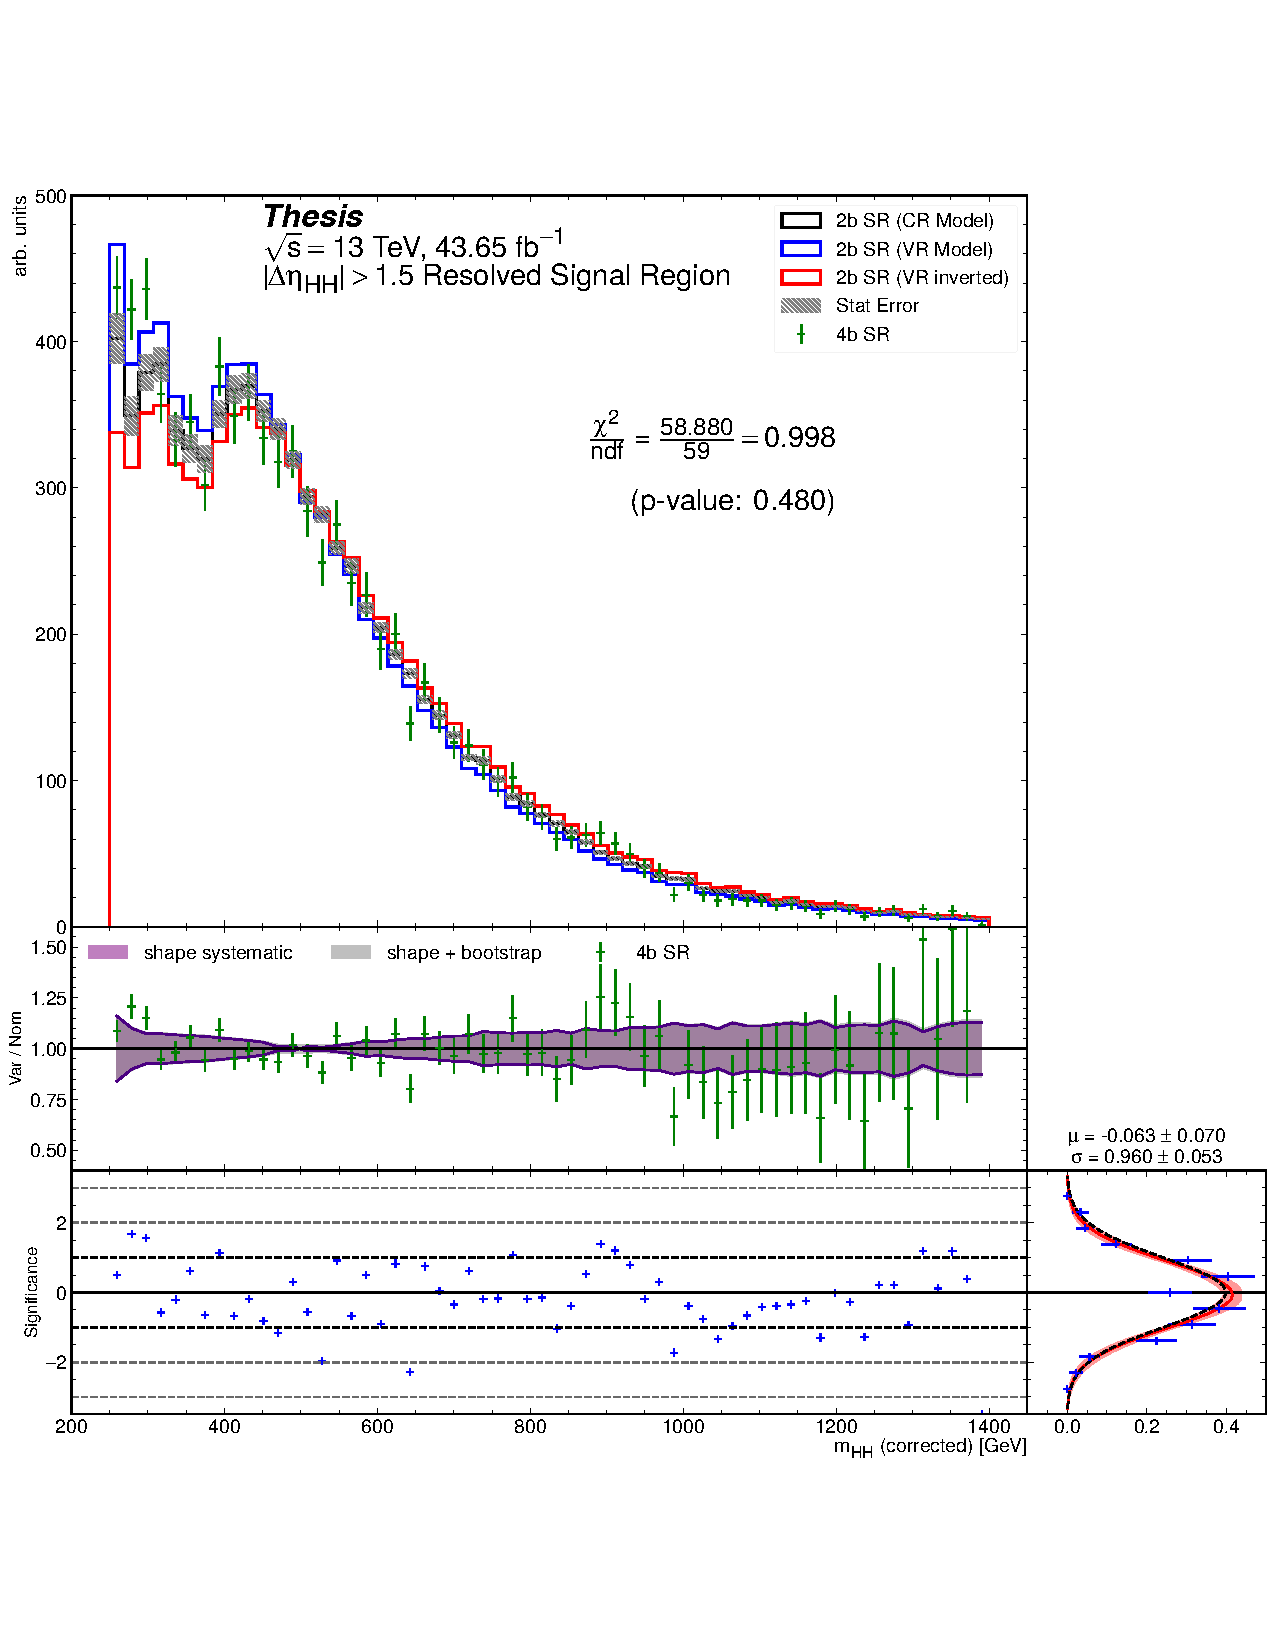
\includegraphics[width=0.65\textwidth]{figures/res-rev-deta.pdf}
	}
	\caption{\label{fig:res-rev-deta} \textbf{Resonant Search}: Performance of the background estimation method in the 
	resonant analysis reversed $\Delta \eta_{HH}$ kinematic signal region. A new background estimate is trained 
	following nominal procedures entirely within the reversed $\Delta \eta_{HH}$ region, and the resulting model, 
	including uncertainties, is compared with $4b$ data in the corresponding signal region. Good agreement is shown. The 
	the quoted $p$-value uses the $\chi^{2}$ test statistic, and demonstrates no evidence that the data differs from the 
	assessed background.}
\end{figure}

\begin{figure}[ht]
  \centering
  \hspace*{-2cm}
  \subfloat{
    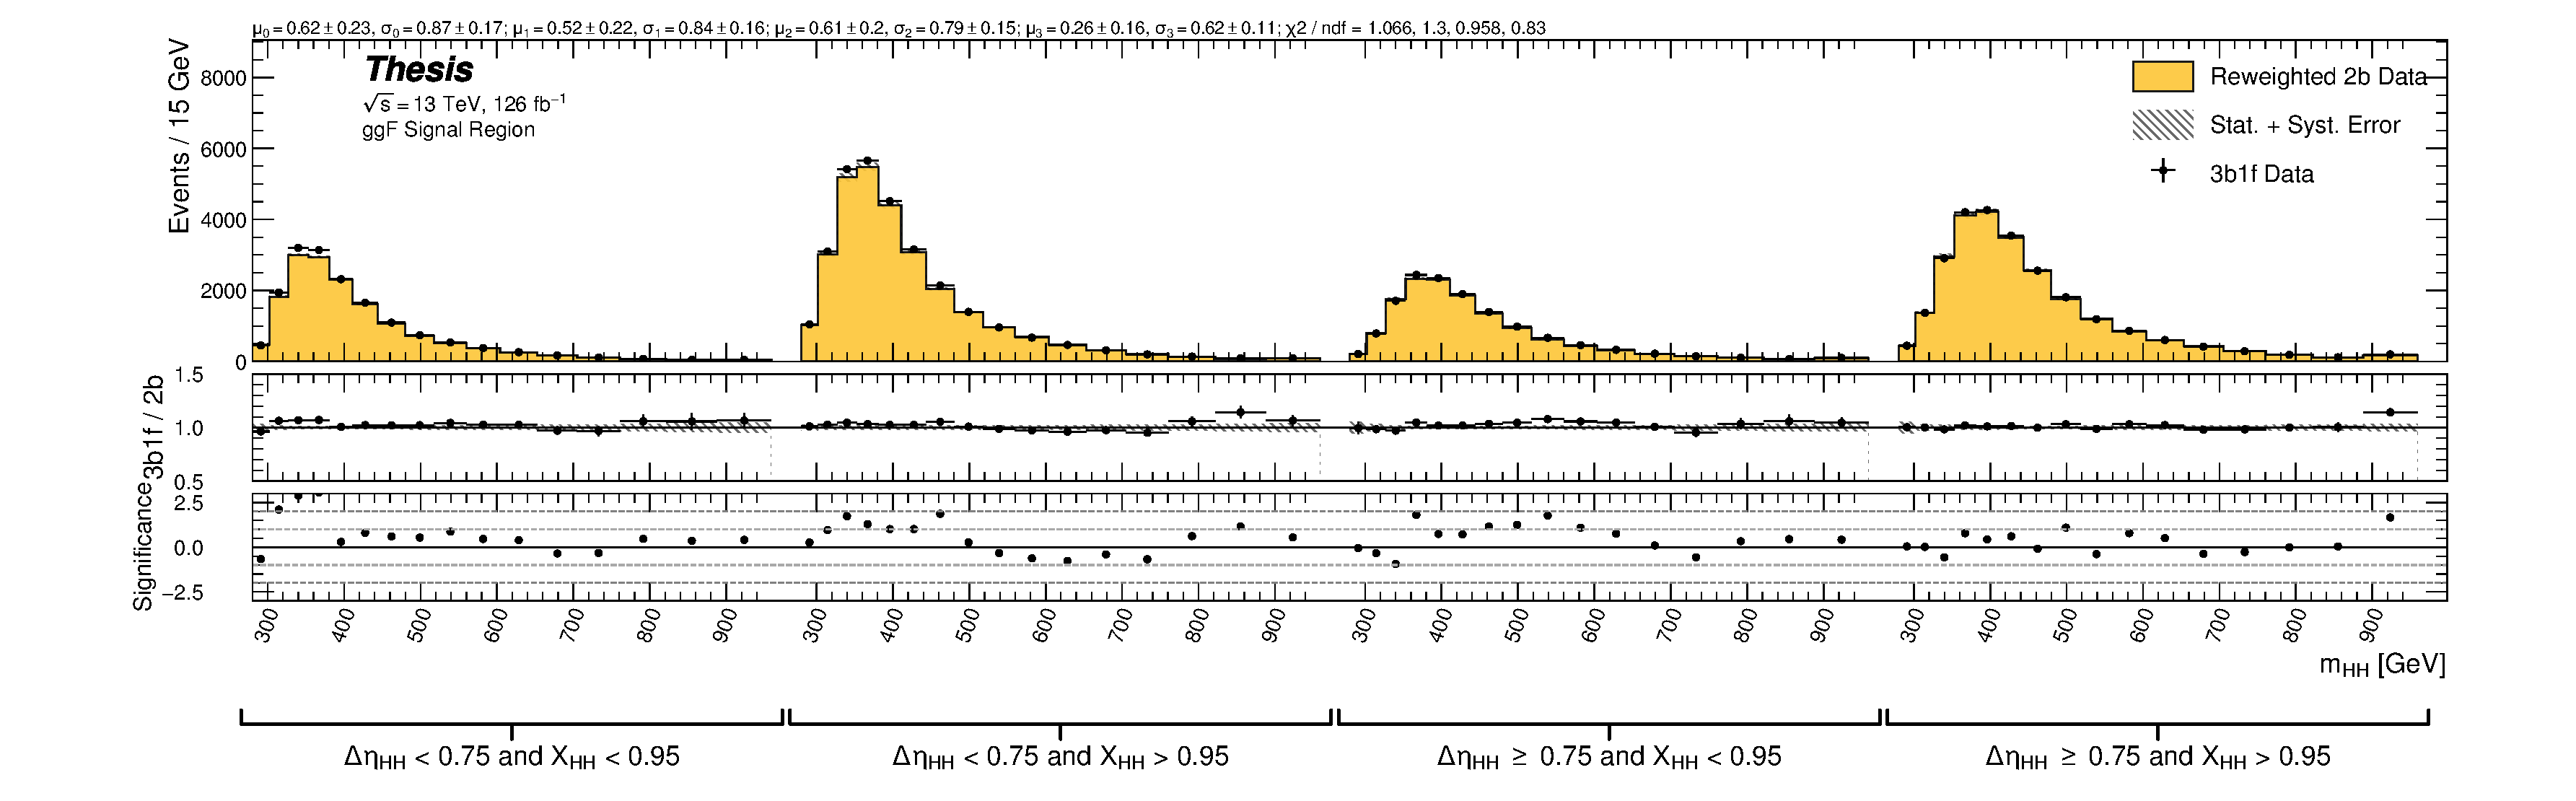
\includegraphics[width=1.2\textwidth]{figures/nonres-3b1f-validation.pdf}
  }
  \caption{\label{fig:nonres-sr-mhh-3b1f} \textbf{Non-resonant Search}: Performance of the background estimation 
  method in the $3b+1$ fail validation region. A new background estimate is trained following nominal procedures 
  but with a reweighting from $2b$ to $3b+1$ fail events. Generally good agreement is seen, though there is some 
  deviation at very low masses in the low $\Delta\eta_{HH}$ low $X_{HH}$ category.}
\end{figure}
